\documentclass[english]{article}

%% Packages pull in extra commands:
%% http://en.wikibooks.org/wiki/LaTeX/Packages

\usepackage{hyperref}
\usepackage[latin9]{inputenc}
\usepackage[letterpaper]{geometry}
\geometry{verbose,tmargin=1in,bmargin=1in,lmargin=1in,rmargin=1in}
\usepackage{amsmath}
\usepackage{amssymb}
\usepackage{graphicx}
\usepackage{float}
\usepackage{array}
\usepackage{enumerate}
\usepackage{tikz}

% New commands serve as shorthand for frequently used command combinations.
\newcommand{\ind}[1]{\mathbf{1}\left(#1\right)}
\newcommand{\bx}{\mathbf{x}}
\newcommand{\E}{\mathbf{E}}

\title{CIS 520, Machine Learning, Fall 2018: Assignment 5}
\author{Shubhankar Patankar}

\begin{document}
\maketitle

{\normalsize \noindent Collaborators: 
 \underline{Simran Arora}} \\

\section{Multiclass Boosting}
\begin{enumerate}

    \item The following definitions are given:
    $$D_1(i) = 1/m$$
    $$D_{t+1}(i) = \frac{D_t(i)exp[-\alpha_t \widetilde{h}_{t,y_i}(x_i)]}{Z_t}$$
    $$F_{T,y_i}(x) = \sum_{t=1}^{T} \alpha_t \widetilde{h}_{t,y_i}(x_i)$$
    At the ($T+1$)-th step, the update equation can be written from definition:
    $$D_{T+1}(i) = \frac{D_T(i)exp\big[-\alpha_T \widetilde{h}_{T,y_i}(x_i)\big]}{Z_T}$$
    Similarly, the update equation at the $T$-th step can be written as follows (citation: Boosting Lecture Notes CIS 520 Spring 2018):
    $$D_{T}(i) = \frac{D_{T-1}(i)exp\big[-\alpha_{T-1} \widetilde{h}_{T-1,y_i}(x_i)\big]}{Z_{T-1}}$$
    Substituting for $D_{T}(i)$ in $D_{T+1}(i)$,
    $$D_{T+1}(i) = \frac{D_{T-1}(i)}{Z_{T+1}Z_T} exp\big[-\alpha_{T-1} \widetilde{h}_{T-1,y_i}(x_i) - \alpha_T \widetilde{h}_{T,y_i}(x_i\big] $$
    Continuing the same process whereby the weights at each previous weak learner are replaced by the update equation for those weights, $D_{T}(i)$ can be written in terms of the initial weights $D_1(i)$.
     \begin{align*}
     D_{T+1}(i)  {}={} & \frac{D_{1}(i)}{Z_1 \dots Z_T} exp\big[-\alpha_{1} \widetilde{h}_{1,y_i}(x_i) - \dots - \alpha_T \widetilde{h}_{T,y_i}(x_i\big] \\
     & = \frac{D_{1}(i)}{\prod_{t=1}^{T} Z_t} exp\bigg[- \sum_{t=1}^{T} \alpha_{t} \widetilde{h}_{t,y_i}(x_i)\bigg] \\
     \end{align*}
     Since by definition $\sum_{t=1}^{T} \alpha_{t} \widetilde{h}_{t,y_i}(x_i) = F_{T,y_i}(x)$ and $D_1(i) = 1/m$,
     $$ D_{T+1}(i) = \frac{\frac{1}{m} e^{- F_{T,y_i}(x)}}{\prod_{t=1}^{T} Z_t}$$ 
    
    \item First consider the case when $H(x_i) = y_i$. Here, $\textbf{1}(H(x_i) \neq y_i)) = 0$. Therefore, the inequality is trivially true since the smallest value that $\textbf{1}(F_{T,y_i} < 0))$ can take is $0$ and $0$ satisfies the inequality, $0 \leq 0$. \newline
    The other case is when $H(x_i) \neq y_i$. We note that $\sum_{k=1}^K F_{T,k}(x_i) = -(K - 2) \sum_{t = 1}^{T}$.  \newline
    \newline \textbf{Proof:} By definition, $F_{T,k}(x_i) = \sum_{t=1}^{T} \alpha_th_{t,k}(x_i)$. 
    $$\therefore \sum_{k=1}^{K} F_{T,k}(x_i) = \sum_{k=1}^{K} \sum_{t=1}^{T} \alpha_t\widetilde{h}_{t,k}(x_i)$$
    $$\sum_{k=1}^{K} F_{T,k}(x_i) =  \sum_{t=1}^{T} \sum_{k=1}^{K} \alpha_t\widetilde{h}_{t,k}(x_i)$$ 
    It is known that $\widetilde{h}_{t,k}(x_i)$ equals $+1$ for one value of $k$ and equals $-1$ for all other values, where $t \in [1..T]$ and $k \in [1..K]$. The summation can then be written as follows:
    $$\sum_{t=1}^{T} \sum_{k=1}^{K} \alpha_t\widetilde{h}_{t,k}(x_i) = \sum_{t=1}^{T} (-1)(K-1)\alpha_t + (+1)\alpha_t = \sum_{t=1}^{T} (-1)(K-2)\alpha_t = -(K-2)\sum_{t=1}^{T} \alpha_t$$
    Returning to the case where, $(H(x_i) \neq y_i)$; $H(x_i)$ returns a class label in $\{1..K\}$. As a result, saying that $H(x_i) \neq y_i$, is equivalent to hypothesizing that $H(x_i) = k$ where $k \neq y_i$. The goal is to prove that in this case as well, $F_{T,y_i}(x_i) < 0$. Assume to contradiction that $H(x_i) \neq y_i$ but $F_{T,y_i}(x_i) > 0$. Noting that since $H(x_i)$ returns the $argmax_k$ as $H(x_i)$, it must be true that $F_{T,k}(x_i) > F_{T,y_i}(x_i)$. And since, $F_{T,y_i}(x_i)$ is assumed to be greater than zero, $F_{T,k}(x_i)$ must also be greater than $0$ under the assumption. 
    Now, using the identity proved above, consider the case when $K = 2$:
    $$F_{T,k_1}(x_i) + F_{T,k_2}(x_i) = \sum_{t=1}^{T} \alpha_t [h_{t,k_1}(x_i) + h_{t,k_2}(x_i)] \leq 0$$  
    When $k_1 = y_i$ and $k_2 = k$ and $F_{T,y_i}(x_i) > 0$ and $F_{T,k}(x_i) > 0$, there is a contradiction to the above inequality since both terms in the summation are positive. From the identity proved above, only one of the two can be positive for the overall sum to be negative. Therefore, we can conclude that if $H(x_i) \neq y_i$ then $F_{T,y_i}(x_i) < 0$, and $\big[\textbf{1}(H(x_i) \neq y_i)) \leq \textbf{1}(F_{T,y_i}(x_i) < 0))\big]$. 
    $$\therefore \textbf{1}(H(x_i) \neq y_i) \leq \textbf{1}(F_{T,y_i}(x_i) < 0)$$

    \item \textbf{Prove that:} $$er_S[H] \leq \frac{1}{m} \sum_{i=1}^{m} e^{-F_{T,y_i}(x_i)} = \prod_{t=1}^{T} Z_t$$
    It is known that the training error of the final classifier $H$ is given by: 
    $$er_S[H] = \frac{1}{m} \sum_{i=1}^{m} \textbf{1}(H(x_i) \neq y_i)$$
    From the inequality proved above in Part $\mathbf{2}$, the error of the final classifier can be rewritten as follows:
    $$er_S[H] \leq \frac{1}{m} \sum_{i=1}^{m} \textbf{1}(F_{T,y_i}(x_i) < 0)$$ Given the fact that $\textbf{1}(u < 0) \leq e^{-u}$, it follows that:
    $$er_S[H] \leq \frac{1}{m} \sum_{i=1}^{m} e^{-F_{T,y_i}(x_i)}$$
    The result from Part $\mathbf{1}$ can be used to prove the equality. Rearranging the result from Part $\mathbf{1}$,
     $$\frac{1}{m} e^{-F_{T,y_i}(x_i)} = \prod_{t=1}^{T} Z_t D_{t+1}(i)$$ 
    Take the sum from $i = 1$ to $i = m$ on both sides to get to the form we want: $$\frac{1}{m}\sum_{i=1}^{m} e^{-F_{T,y_i}(x_i)} = \sum_{i=1}^{m}\prod_{t=1}^{T} Z_t D_{t+1}(i)$$
    $$\therefore \frac{1}{m}\sum_{i=1}^{m} e^{-F_{T,y_i}(x_i)} = \prod_{t=1}^{T} Z_t \sum_{i=1}^{m} D_{t+1}(i)$$
    Since $\sum_{i=1}^{m} D_{t+1}(i) = 1$,
    $$\frac{1}{m}\sum_{i=1}^{m} e^{-F_{T,y_i}(x_i)} = \prod_{t=1}^{T} Z_t $$
    
    \item The goal is to prove that for a given choice of $\alpha_t$, $Z_t = 2\sqrt{er_t(1 - er_t)}$. \\
    From the AdaBoost algorithm the following equations are known: 
    $$\alpha_t = \frac{1}{2} ln\bigg(\frac{1 - er_t}{er_t}\bigg) = ln\bigg(\frac{1 - er_t}{er_t}\bigg)^{\frac{1}{2}}$$
    $$Z_t = \sum_{j=1}^{m} D_t(j) e^{-\alpha_t\widetilde{h}_{t,k}(x_j)}$$ 
    It is also known that $\widetilde{h}_{t,y_j}(x_j) = 1$ if $h_t(x_j) = y_j$ and $\widetilde{h}_{t,y_j}(x_j) = -1$ otherwise. Substituting for $\widetilde{h}_{t,y_j}(x_j)$ and $\alpha_t$ and using $\textbf{1}(\widetilde{h}_{t,y_j}(x_j) = y_j)$ as an indicator variable (citation: Boosting Lecture Notes CIS 520 Spring 2018): 
    $$Z_t = \sum_{j=1}^{m} D_t(j) e^{-\alpha_t\widetilde{h}_{t,k}(x_j)}$$
    $$Z_t = \sum_{j=1}^{m} D_t(j) e^{-\alpha_t[\textbf{1}(\widetilde{h}_{t,y_j}(x_j) = y_j) - \textbf{1}(\widetilde{h}_{t,y_j}(x_j) \neq y_j)]}$$
    $$Z_t = \sum_{j=1}^{m} \bigg[D_t(j) e^{-\alpha_t[\textbf{1}(\widetilde{h}_{t,y_j}(x_j) = y_j)]} + D_t(j)e^{\alpha_t[\textbf{1}(\widetilde{h}_{t,y_j}(x_j) \neq y_j)]}\bigg]$$
     $$Z_t = \sum_{j=1}^{m} \bigg[ D_t(j) e^{-\alpha_t[\textbf{1}(\widetilde{h}_{t,y_j}(x_j) = y_j)]} + D_t(j)e^{\alpha_t[\textbf{1}(\widetilde{h}_{t,y_j}(x_j) \neq y_j)]}\bigg]$$
     Note that: 
     $$e^{\alpha_t[\textbf{1}(\widetilde{h}_{t,y_j}(x_j) \neq y_j)]} = e^{ln\big(\frac{1 - er_t}{er_t}\big)^{\frac{1}{2}}[\textbf{1}(\widetilde{h}_{t,y_j}(x_j) \neq y_j)]} = \sqrt{\frac{1 - er_t}{er_t}}(\textbf{1}(\widetilde{h}_{t,y_j}(x_j) \neq y_j)$$ 
     Also note that:
     $$e^{-\alpha_t} = e^{-ln\big(\frac{1 - er_t}{er_t}\big)^{\frac{1}{2}}} = e^{ln\big(\frac{1 - er_t}{er_t}\big)^{\frac{-1}{2}}} = \sqrt{\frac{er_t}{1 - er_t}}$$
     $Z_t$ can then be re-written as follows: 
     $$Z_t = \sqrt{\frac{ er_t}{1-er_t}}\sum_{j=1}^{m} D_t(j) [\textbf{1}(\widetilde{h}_{t,y_j}(x_j) = y_j)] + \sqrt{\frac{1 - er_t}{er_t}}\sum_{j=1}^{m} D_t(j)[\textbf{1}(\widetilde{h}_{t,y_j}(x_j) \neq y_j)]$$
     It is known that the training error of the $t$-th classifier is defined as $er_t[h] = \sum_{j=1}^{m} D_t(j) \textbf{1}(h(x_j) \neq y_j)$. 
     $$\therefore Z_t = \sqrt{\frac{er_t}{1 - er_t}}(1 - er_t)+ \sqrt{\frac{1 - er_t}{er_t}}(er_t)$$
     $$Z_t = \sqrt{\frac{er_t}{1 - er_t}(1 - er_t)^2} + \sqrt{\frac{1 - er_t}{er_t}(er_t)^2}$$
     $$Z_t = \sqrt{(er_t)(1 - er_t)} + \sqrt{(1 - er_t)(er_t)}$$
     $$\therefore Z_t = 2\sqrt{(er_t)(1 - er_t)}$$

    \item \textbf{Prove that:} $er_S[H] \leq e^{-2T\gamma^2}$ when $er_t \leq \frac{1}{2} - \gamma$ for all $t$ where $0 < \gamma \leq \frac{1}{2}$. \\
    It was shown in Part $\mathbf{2}$ that $\textbf{1}(H(x_i) \neq y_i)) \leq \textbf{1}(F_{T,y_i}(x_i) < 0))$. \\
    It was shown in Part $\mathbf{3}$ that $er_S[H] \leq \frac{1}{m} \sum_{i=1}^{m}\textbf{1}(H(x_i) \neq y_i) = \prod_{t=1}^{T} Z_t$. 
    As a result, it is known that:
     $$er_S[H]  \leq \prod_{t=1}^T Z_t$$ 
     Using the result derived in Part $\mathbf{4}$: 
     $$er_S[H]  \leq \prod_{t=1}^T 2\sqrt{(er_t)(1 - er_t)}$$ 
     % Since $er_t \leq \frac{1}{2} - \gamma$ for all $t$ where $0 < \gamma \leq \frac{1}{2}$. 
     As $er_t$ increases on the interval from $0$ to $1/2$, $\sqrt{(er_t)(1 - er_t)}$ also increases (citation: Boosting Lecture Notes CIS 520 Spring 2018). With this information and with $er_t \leq \frac{1}{2} - \gamma$ for all $t$ where $0 < \gamma \leq \frac{1}{2}$, the above inequality can be re-written as follows: 
     % Since as $er_t$ gets bigger, the result of $x = er_t(1-er_t)$ gets bigger, we know the value of $x$ is maximized when $er_t = \frac{1}{2} - \gamma$. 
    $$er_S[H] \leq \prod_{t=1}^T 2\sqrt{\bigg(\frac{1}{2} - \gamma\bigg)\bigg(1 - \frac{1}{2} + \gamma\bigg)}$$
    $$er_S[H] \leq \prod_{t=1}^T 2\sqrt{\frac{1}{4} - \gamma^2}$$
    $$\therefore er_S[H] \leq 2^T\bigg(\sqrt{\frac{1}{4} - \gamma^2}\bigg)^T = 2^T\bigg(\frac{1}{4} - \gamma^2\bigg)^{\frac{T}{2}} = (1 - 4\gamma^2)^{\frac{T}{2}}$$
    Since it is known $1 - x \leq e^{-x}$: 
    $$er_S[H] \leq (1 - 4\gamma^2)^{\frac{T}{2}} \leq e^{(2T\gamma^2)}$$ 
     
\end{enumerate}

\newpage
\section{Perceptron vs. Winnow}
The number of mistakes made by the perceptron algorithm is at most:
$$\frac{R_2^2 ||\mathbf{u}||_2^2}{\gamma^2}$$
where, $R_2 = max_{1\leq t\leq T} ||\mathbf{x_t}||_2$. (citation: Online Learning and Perceptron Lecture Notes CIS 520 Fall 2017) \\
The number of mistakes made by the winnow algorithm is at most:
$$2\bigg(\frac{R_\infty^2 ||\mathbf{u}||_1^2}{\gamma^2}\bigg) ln(d)$$
where, $R_\infty \geq ||\mathbf{x_t}||_\infty$ for all trials $t$. 
\begin{enumerate}
    \item For perceptron, $R_2 = max_{1\leq t\leq T} ||\mathbf{x_t}||_2 \implies R_2 = \sqrt d$, since $\mathbf{x_t}$ is $\pm1$ $d$ times. $\mathbf{u}$ has $k$ non-zero entries $\implies ||\mathbf{u}||_2^2 = k$.  
    $$\therefore bound_{perceptron} = \frac{dk}{\gamma^2}$$
    For winnow, $R_\infty \geq ||\mathbf{x_t}||_\infty \implies R_\infty \geq 1$, since the largest element in $\mathbf{x_t}$ is $1$. Since, $\mathbf{u}$ has $k$ non-zero elements,  $||\mathbf{u}||_1 = k$.
    $$\therefore bound_{winnow} = \frac{2k^2}{\gamma^2}ln(d)$$
    The ratio of the maximum number of errors made by winnow to the maximum number of errors made by perceptron is:
    $$\frac{bound_{winnow}}{bound_{perceptron}} = \frac{2kln(d)}{d^2}$$
    The numerator is smaller than the denominator since $ln(d) < d$ and $k << d$. Therefore, in the case where the target vector $\mathbf{u}$ is sparse ($k << d$) and the feature vector $\mathbf{x}$ is dense, winnow outperforms perceptron. 
    \item For perceptron, $R_2 = max_{1\leq t\leq T} ||\mathbf{x_t}||_2 \implies R_2 = \sqrt k$, since each $\mathbf{x_t}$ has $k << d$ non-zero entries. \\
    It is given that the dense weight vector $\mathbf{u}$ has L1 norm $||\mathbf{u}||_1 = d$ and L2 norm $||\mathbf{u}||_2 \leq 2\sqrt d$. 
    $$\therefore bound_{perceptron} = \frac{4kd}{\gamma^2}$$
    For winnow, even in the case with a sparse feature vector $\mathbf{x_t}$, the greatest value in $\mathbf{x_t}$ is $1$ and as a result $R_\infty \geq 1$. 
    $$\therefore bound_{winnow} = \frac{2d^2}{\gamma^2}ln(d)$$
    The ratio of the maximum number of errors made by winnow to the maximum number of errors made by perceptron is:
    $$\frac{bound_{winnow}}{bound_{perceptron}} = \frac{d \times ln(d)}{2k}$$
    The denominator is smaller than the numerator since $k << d$, implying that the perceptron algorithm is better when the target vector is dense and the feature vector sparse. 
    \item If the feature vector is non-negative, the prediction step in the winnow algorithm ($\hat{y} = sign(\mathbf{w_t}^T \mathbf{x_t})$) would return either a $0$ or a $1$. But since the true labels are $\pm1$, the '$0$'-predicted labels would always be presumed to have been misclassified. The algorithm would work if the true labels were also changed to be $0$ or $1$ instead of $\pm1$. 
\end{enumerate}

\section{Principal Component Analysis}
\begin{enumerate}
    \item 12000-th Data Point \\ \\
    \textbf{Code to generate 12000th data point}
    \begin{verbatim}
    load('MNIST_train.mat')
    mean_column = mean(X_train, 1);
    mean = repmat(mean_column, 12000, 1);
    mc_X_train = X_train - mean;
    testImage = imrotate(fliplr(reshape(mc_X_train(end,:), 28, 28)),90);
    figure;
    colormap(gray);
    imagesc(testImage)
    \end{verbatim}
    
    \begin{figure}[H]
    \centering
    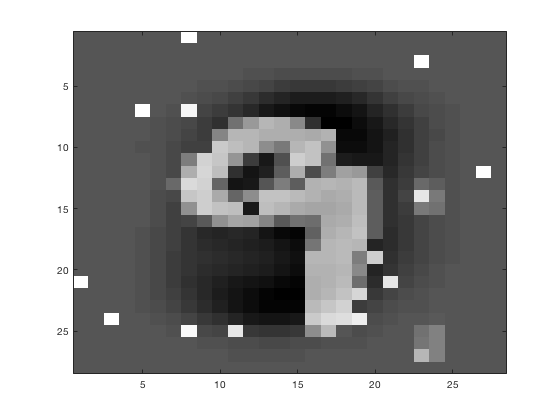
\includegraphics[scale = 0.45]{fig31}
    \caption{Regenerated Example Image}
    \label{fig:fig31}
    \end{figure}
    
    \newpage
    \item PC Vectors as Images
    \begin{figure}[H]
    \centering
    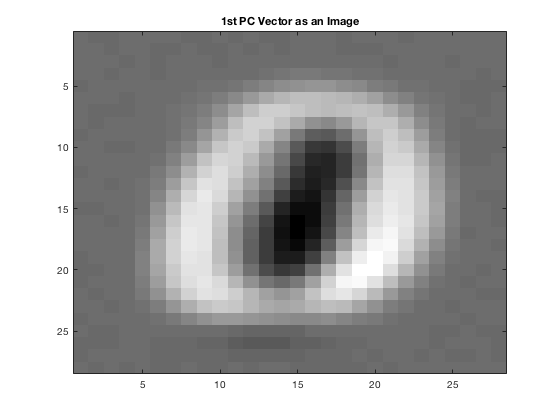
\includegraphics[scale = 0.5]{fig321}
    \caption{First PC Vector as an Image}
    \label{fig:fig321}
    \end{figure}
    
    \begin{figure}[H]
    \centering
    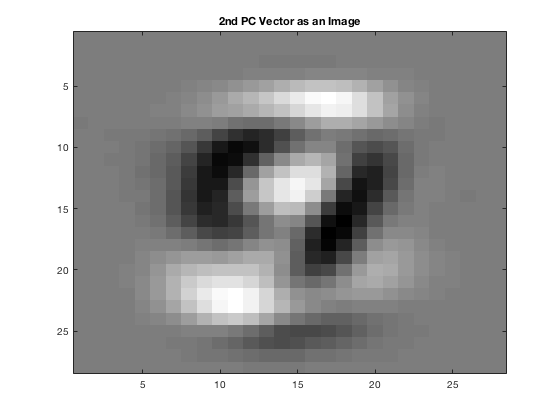
\includegraphics[scale = 0.5]{fig322}
    \caption{Second PC Vector as an Image}
    \label{fig:fig322}
    \end{figure}
    
    \begin{figure}[H]
    \centering
    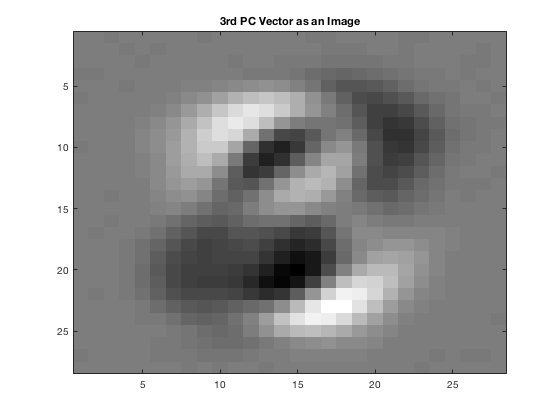
\includegraphics[scale = 0.5]{fig323}
    \caption{Third PC Vector as an Image}
    \label{fig:fig323}
    \end{figure}
    
    The images of the PC Vectors make sense, since they resemble the digits of the MNIST dataset in some abstract sense. Any digit in the original dataset can be expressed as a linear combination of the PC vectors. In this sense, the PC vectors act as the "eigendigits" and the above figures confirm their vague resemblance to true digits. 
    
    \item Digits $0$ and $7$ Along PC Directions
    \begin{figure}[H]
    \centering
    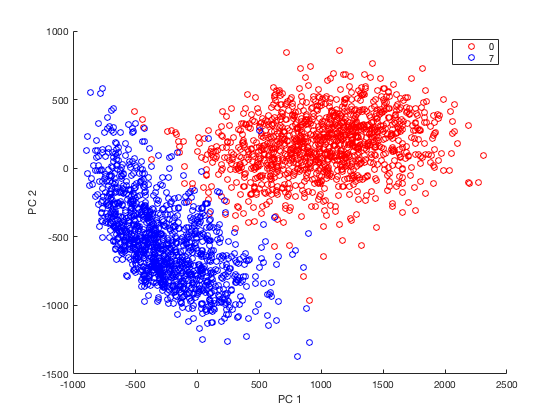
\includegraphics[scale = 0.6]{fig331}
    \caption{1st and 2nd PC Dimensions}
    \label{fig:fig322}
    \end{figure}
    
    In the first 2 PC directions, the digits labelled $0$ and $7$ have almost no overlap. Since the variance of the true data is captured in a descending order of PCs, it makes sense that most of the difference in two labels should be encapsulated by the first few principal components. The lack of overlap in the figure is an indicator of the high variance explained by the first two PCs. 
    
    \begin{figure}[H]
    \centering
    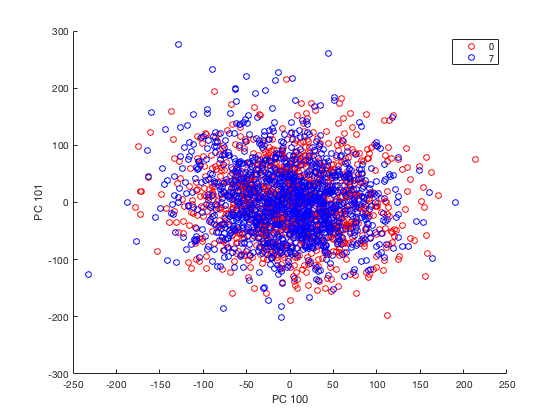
\includegraphics[scale = 0.6]{fig332}
    \caption{100th and 101st PC Dimensions}
    \label{fig:fig323}
    \end{figure}
    
    As we move towards PCs that explain lower and lower amounts of variance in the true data, it makes sense that two distinct labels start becoming indistinguishable in the higher PC directions. These PC directions are not good at separating the data, which is equivalent to saying that these directions explain less variance of the true data. 
    
    \newpage
    \item Reconstruction Accuracy
    \begin{figure}[H]
    \centering
    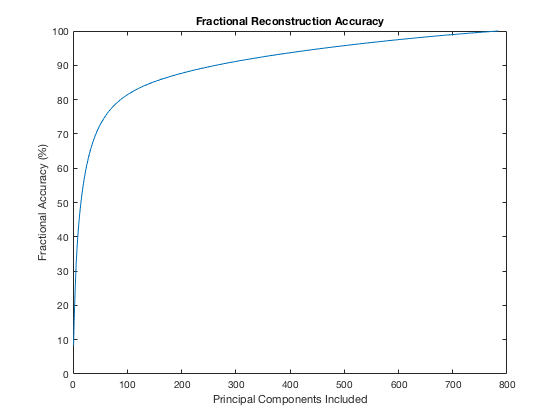
\includegraphics[scale = 0.65]{fig341}
    \caption{Reconstruction Accuracy}
    \label{fig:fig341}
    \end{figure}
    
    Table 1: \%Variance Explained by PCs
    \begin{figure}[H]
    \centering
    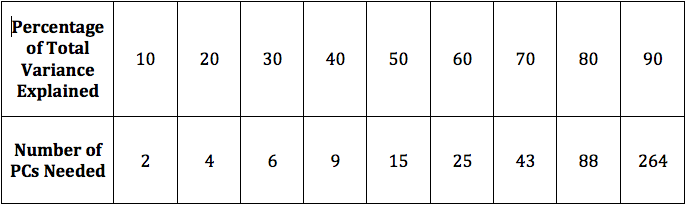
\includegraphics[scale = 0.5]{fig342}
    \label{fig:fig342}
    \end{figure}
    
    \newpage
    \item Reconstructed Example Digits from the MNIST Dataset
    \begin{figure}[H]
    \centering
    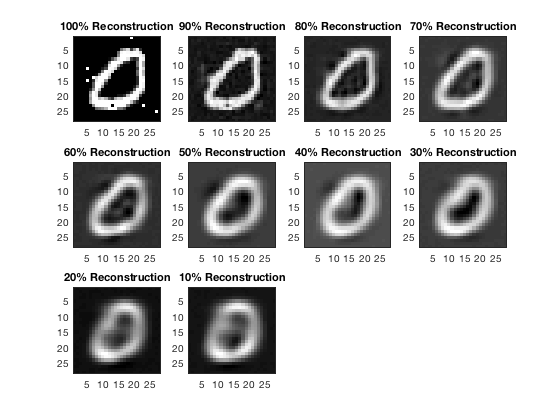
\includegraphics[scale = 0.65]{fig351}
    \caption{500th Example}
    \label{fig:fig321}
    \end{figure}
    
    \begin{figure}[H]
    \centering
    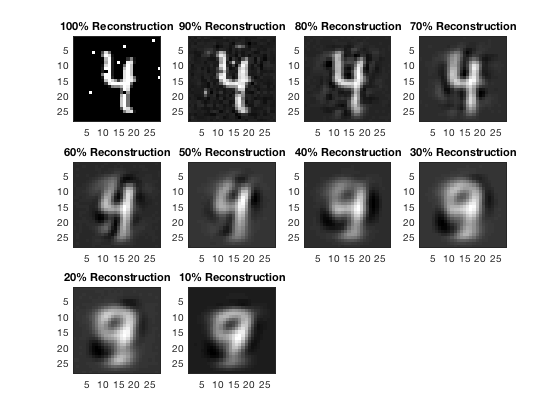
\includegraphics[scale = 0.65]{fig352}
    \caption{6000th Example}
    \label{fig:fig322}
    \end{figure}
    
    \begin{figure}[H]
    \centering
    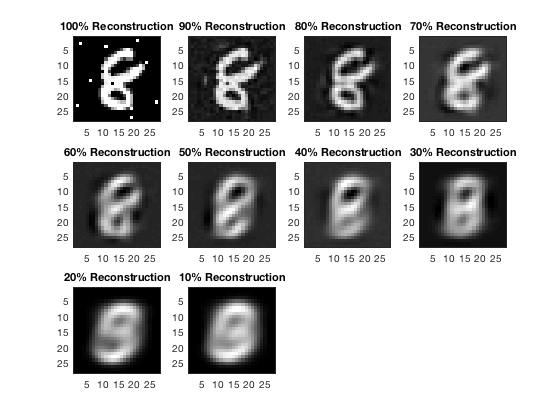
\includegraphics[scale = 0.65]{fig353}
    \caption{10000th Example}
    \label{fig:fig323}
    \end{figure}
    
    \item Reconstruction Accuracy: Autoencoders vs PCA
    \begin{figure}[H]
    \centering
    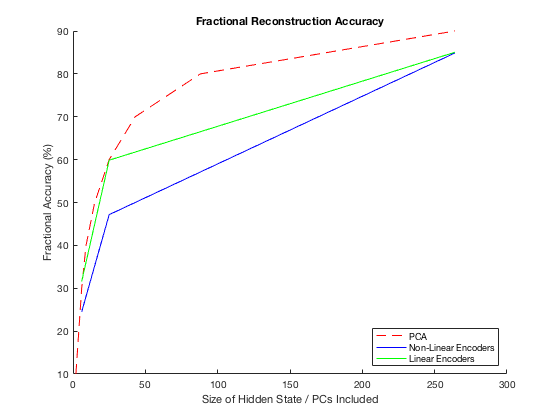
\includegraphics[scale = 0.65]{fig36}
    \caption{10000th Example}
    \label{fig:fig36}
    \end{figure}
    
    From the above figure, it is seen that PCA outperforms the non-linear autoencoders in its ability to reconstruct the data. It is less clear as to whether PCA is also better than the linear encoders. In theory, the error function has a unique global minimum at which a linearly activated network performs a projection onto the lower dimensional vector space spanned by the principal component vectors. This is a result that follows by noting that the PCA and the neural network are minimizing the same sum-of-squares error function (citation: Bishop pg.593). It is not surprising, therefore, that PCA and linear autoencoders have almost the same results for data points where results for both approaches exist. 
    It is also seen that PCA/linear functions are better than non-linear encoder/decoder functions in terms of their reconstruction accuracies. In theory, using non-linear activation functions should not cause us to be worse off than using linear activation functions, since non-linear functions also perform a projection onto the space spanned by the PC vectors (citation: Bishop pg.593). However, since the problem is now a nonlinear optimization problem, the error function is not of the sum-of-squares form. Computationally costlier methods might be needed to solve such a problem with the added risk of being stuck in a suboptimal local minimum (citation: Bishop pg.595). The intensity of the computation suggests that more iterations might be needed for convergence in the case of non-linear activation functions. Perhaps, the reason for the underperformance of the non-linear activation functions in this case is that the encoders were not trained for a sufficient number of epochs. 
    
    \item Adding more layers to the encoder/decoder is equivalent to increasing the complexity of the model. More layers might lead to better fits to the training data and therefore higher reconstruction accuracies. However, the lack of any regularization also runs the risk of overfitting to the training samples.
    Additionally, based on the discussion above, another factor to consider when layers are added, is whether the layers are linearly or non-linearly activated. 
    Including non-linear activation functions might cause the same problems as described in Part \textbf{6} above for the non-linear encoders. The solution might get stuck in a suboptimal local minimum and the network might have to be trained for longer. 
    
\end{enumerate}

\newpage
\section{Eigenvectors}
Using Singular Value Decomposition, $X = U{\Lambda}V^T \implies X^T = V{\Lambda}^TU^T$. 
$$\therefore X^TX = V{\Lambda}^TU^TU{\Lambda}V^T$$
Since $UU^T = VV^T = I$, 
$$X^TX = V{\Lambda}^T{\Lambda}V^T$$
\begin{enumerate}
\item From lecture (October 17, 2018), it is known that $X^+ = (X^TX)^{-1}X^T$ is a solution to the least-squares problem.
Re-writing $X$ and $X^T$ in terms of the singular value decomposition gives,
$$(X^TX)^{-1}X^T = (V{\Lambda}^T{\Lambda}V^T)^{-1}(V{\Lambda}^TU^T)$$
In the above equation, the matrices can be broken down into blocks such that ${\Lambda}_p$ is a square matrix of dimensions $p \times p$. The terms in ${\Lambda}$ from rows $n+1$ to $p$ are $0$ and disappear. Since, ${\Lambda}_p$ is a square diagonal matrix, its inverse exists. 
The resulting non-zero remnant portion can be written as follows:
$$(X^TX)^{-1}X^T = {{V_p}^T}^{-1}{\Lambda_p}^{-1}{{\Lambda_p}^T}^{-1}{V_p}^{-1}V_p{\Lambda_p}^T{U_p}^T$$
$$(X^TX)^{-1}X^T = V_p{\Lambda_p}^{-1}{U_p}^T$$
$$\therefore X^+ = (X^TX)^{-1}X^T = V_p{\Lambda_p}^{-1}{U_p}^T$$
If $X^+ = (X^TX)^{-1}X^T$ is a solution to the least squares problem, from the above equality, $V_p{\Lambda_p}^{-1}{U_p}^T$ is equivalently a solution. 
When $k = p$, $V_k{\Lambda_k}^{-1}{U_k}^T$ is equal to $V_p{\Lambda_p}^{-1}{U_p}^T$ and therefore is also a solution to the least squares problem. 

% \item 
% $$X\hat{w} = y$$
% Multiplying both sides by $X^T$,
% $$X^TX\hat{w} = X^Ty$$
% $$\therefore V{\Lambda}^T{\Lambda}V^T\hat{w} = V\Lambda^TU^Ty$$
% Since $X$ is full rank, $X^TX$ is full rank and therefore invertible. The inverse of $V{\Lambda}^T{\Lambda}V^T$ exists. 
% $$\therefore \hat{w} = (V{\Lambda}^T{\Lambda}V^T)^{-1}(V{\Lambda}^TU^T)y$$
% $$\therefore \hat{w} = {V^T}^{-1}{\Lambda}^{-1}{{\Lambda}^T}^{-1}V^{-1}V{\Lambda}^TU^Ty$$
% $$\therefore \hat{w} = {V^T}^{-1}{\Lambda}^{-1}U^Ty$$
% $$\therefore \hat{w} = V{\Lambda}^{-1}U^Ty$$
% $\because V{\Lambda}^{-1}U^T = X^+ \implies \hat{w} = X^+y$, solves problem $X\hat{w} = y$. \\
% The least squares problem is solved when $||y - Xw||_2^2$ is minimized. \\
% $y$ can be replaced by $X\hat{w}$.
% Both terms in $||X\hat{w} - Xw||_2^2$ equal $y$ implying $||y - Xw||_2^2 = 0$. The smallest the L2 norm can be is $0$. Therefore $\hat{w} = X^+y$ solves the least squares problem. 

\item 
$$X = U{\Lambda}V^T$$
Multiplying both sides on the right by $V$,
$$XV = U{\Lambda}V^TV$$
$$\therefore XV = U{\Lambda}$$
Multiplying both sides on the left by $X^T$,
$$X^TXV = X^TU{\Lambda}$$
The singular values on the diagonal of $\Lambda$ are the square roots of the eigenvalues of $X^TX$ (citation: Principal Component Analysis Lecture Notes CIS 520 Spring 2018). This implies that $X^TXV = LV$ can also be written as $X^TXV = {\Lambda}^2V$, where $L$ is a matrix that has the eigenvalues of $X^TX$ on its diagonal. 
$$\therefore X^TXV = X^TU{\Lambda} = {\Lambda}^2V$$
Since $X^TU{\Lambda} = {\Lambda}^2V$, it follows that any eigenvector $v_i$ can be obtained by performing the following computation:
$$v_i = \frac{X^Tu_i}{\lambda}$$
In the above equation, $\lambda$ is a singular value corresponding to the associated eigenvalue of $X^TX$. By obtaining the largest eigenvectors $u_i$ of $XX^T$ using tools such as the Power Method or Fast Randomized SV, the eigenvectors of $X^TX$ can be computed from the relationship above. 

\end{enumerate}

\end{document}